\documentclass[11pt,a4paper]{report}
\usepackage[textwidth=37em,vmargin=30mm]{geometry}
\usepackage{calc,xunicode,amsmath,amssymb,paralist,enumitem,tabu,booktabs,datetime2,xeCJK,xeCJKfntef,listings}
\usepackage{tocloft,fancyhdr,tcolorbox,xcolor,graphicx,eso-pic,xltxtra,xelatexemoji}

\newcommand{\envyear}[0]{2025}
\newcommand{\envdatestr}[0]{2025-10-22}
\newcommand{\envfinaldir}[0]{webdb/2025/20251022/final}

\usepackage[hidelinks]{hyperref}
\hypersetup{
    colorlinks=false,
    pdfpagemode=FullScreen,
    pdftitle={Web Digest - \envdatestr}
}

\setlength{\cftbeforechapskip}{10pt}
\renewcommand{\cftchapfont}{\rmfamily\bfseries\large\raggedright}
\setlength{\cftbeforesecskip}{2pt}
\renewcommand{\cftsecfont}{\sffamily\small\raggedright}

\setdefaultleftmargin{2em}{2em}{1em}{1em}{1em}{1em}

\usepackage{xeCJK,xeCJKfntef}
\xeCJKsetup{PunctStyle=plain,RubberPunctSkip=false,CJKglue=\strut\hskip 0pt plus 0.1em minus 0.05em,CJKecglue=\strut\hskip 0.22em plus 0.2em}
\XeTeXlinebreaklocale "zh"
\XeTeXlinebreakskip = 0pt


\setmainfont{Brygada 1918}
\setromanfont{Brygada 1918}
\setsansfont{IBM Plex Sans}
\setmonofont{JetBrains Mono NL}
\setCJKmainfont{Noto Serif CJK SC}
\setCJKromanfont{Noto Serif CJK SC}
\setCJKsansfont{Noto Sans CJK SC}
\setCJKmonofont{Noto Sans CJK SC}

\setlength{\parindent}{0pt}
\setlength{\parskip}{8pt}
\linespread{1.15}

\lstset{
	basicstyle=\ttfamily\footnotesize,
	numbersep=5pt,
	backgroundcolor=\color{black!5},
	showspaces=false,
	showstringspaces=false,
	showtabs=false,
	tabsize=2,
	captionpos=b,
	breaklines=true,
	breakatwhitespace=true,
	breakautoindent=true,
	linewidth=\textwidth
}






\newcommand{\coverpic}[2]{
    % argv: itemurl, authorname
    Cover photo by #2~~(\href{#1}{#1})
}
\newcommand{\makeheader}[0]{
    \begin{titlepage}
        % \newgeometry{hmargin=15mm,tmargin=21mm,bmargin=12mm}
        \begin{center}
            
            \rmfamily\scshape
            \fontspec{BaskervilleF}
            \fontspec{Old Standard}
            \fontsize{59pt}{70pt}\selectfont
            WEB\hfill DIGEST
            
            \vfill
            % \vskip 30pt
            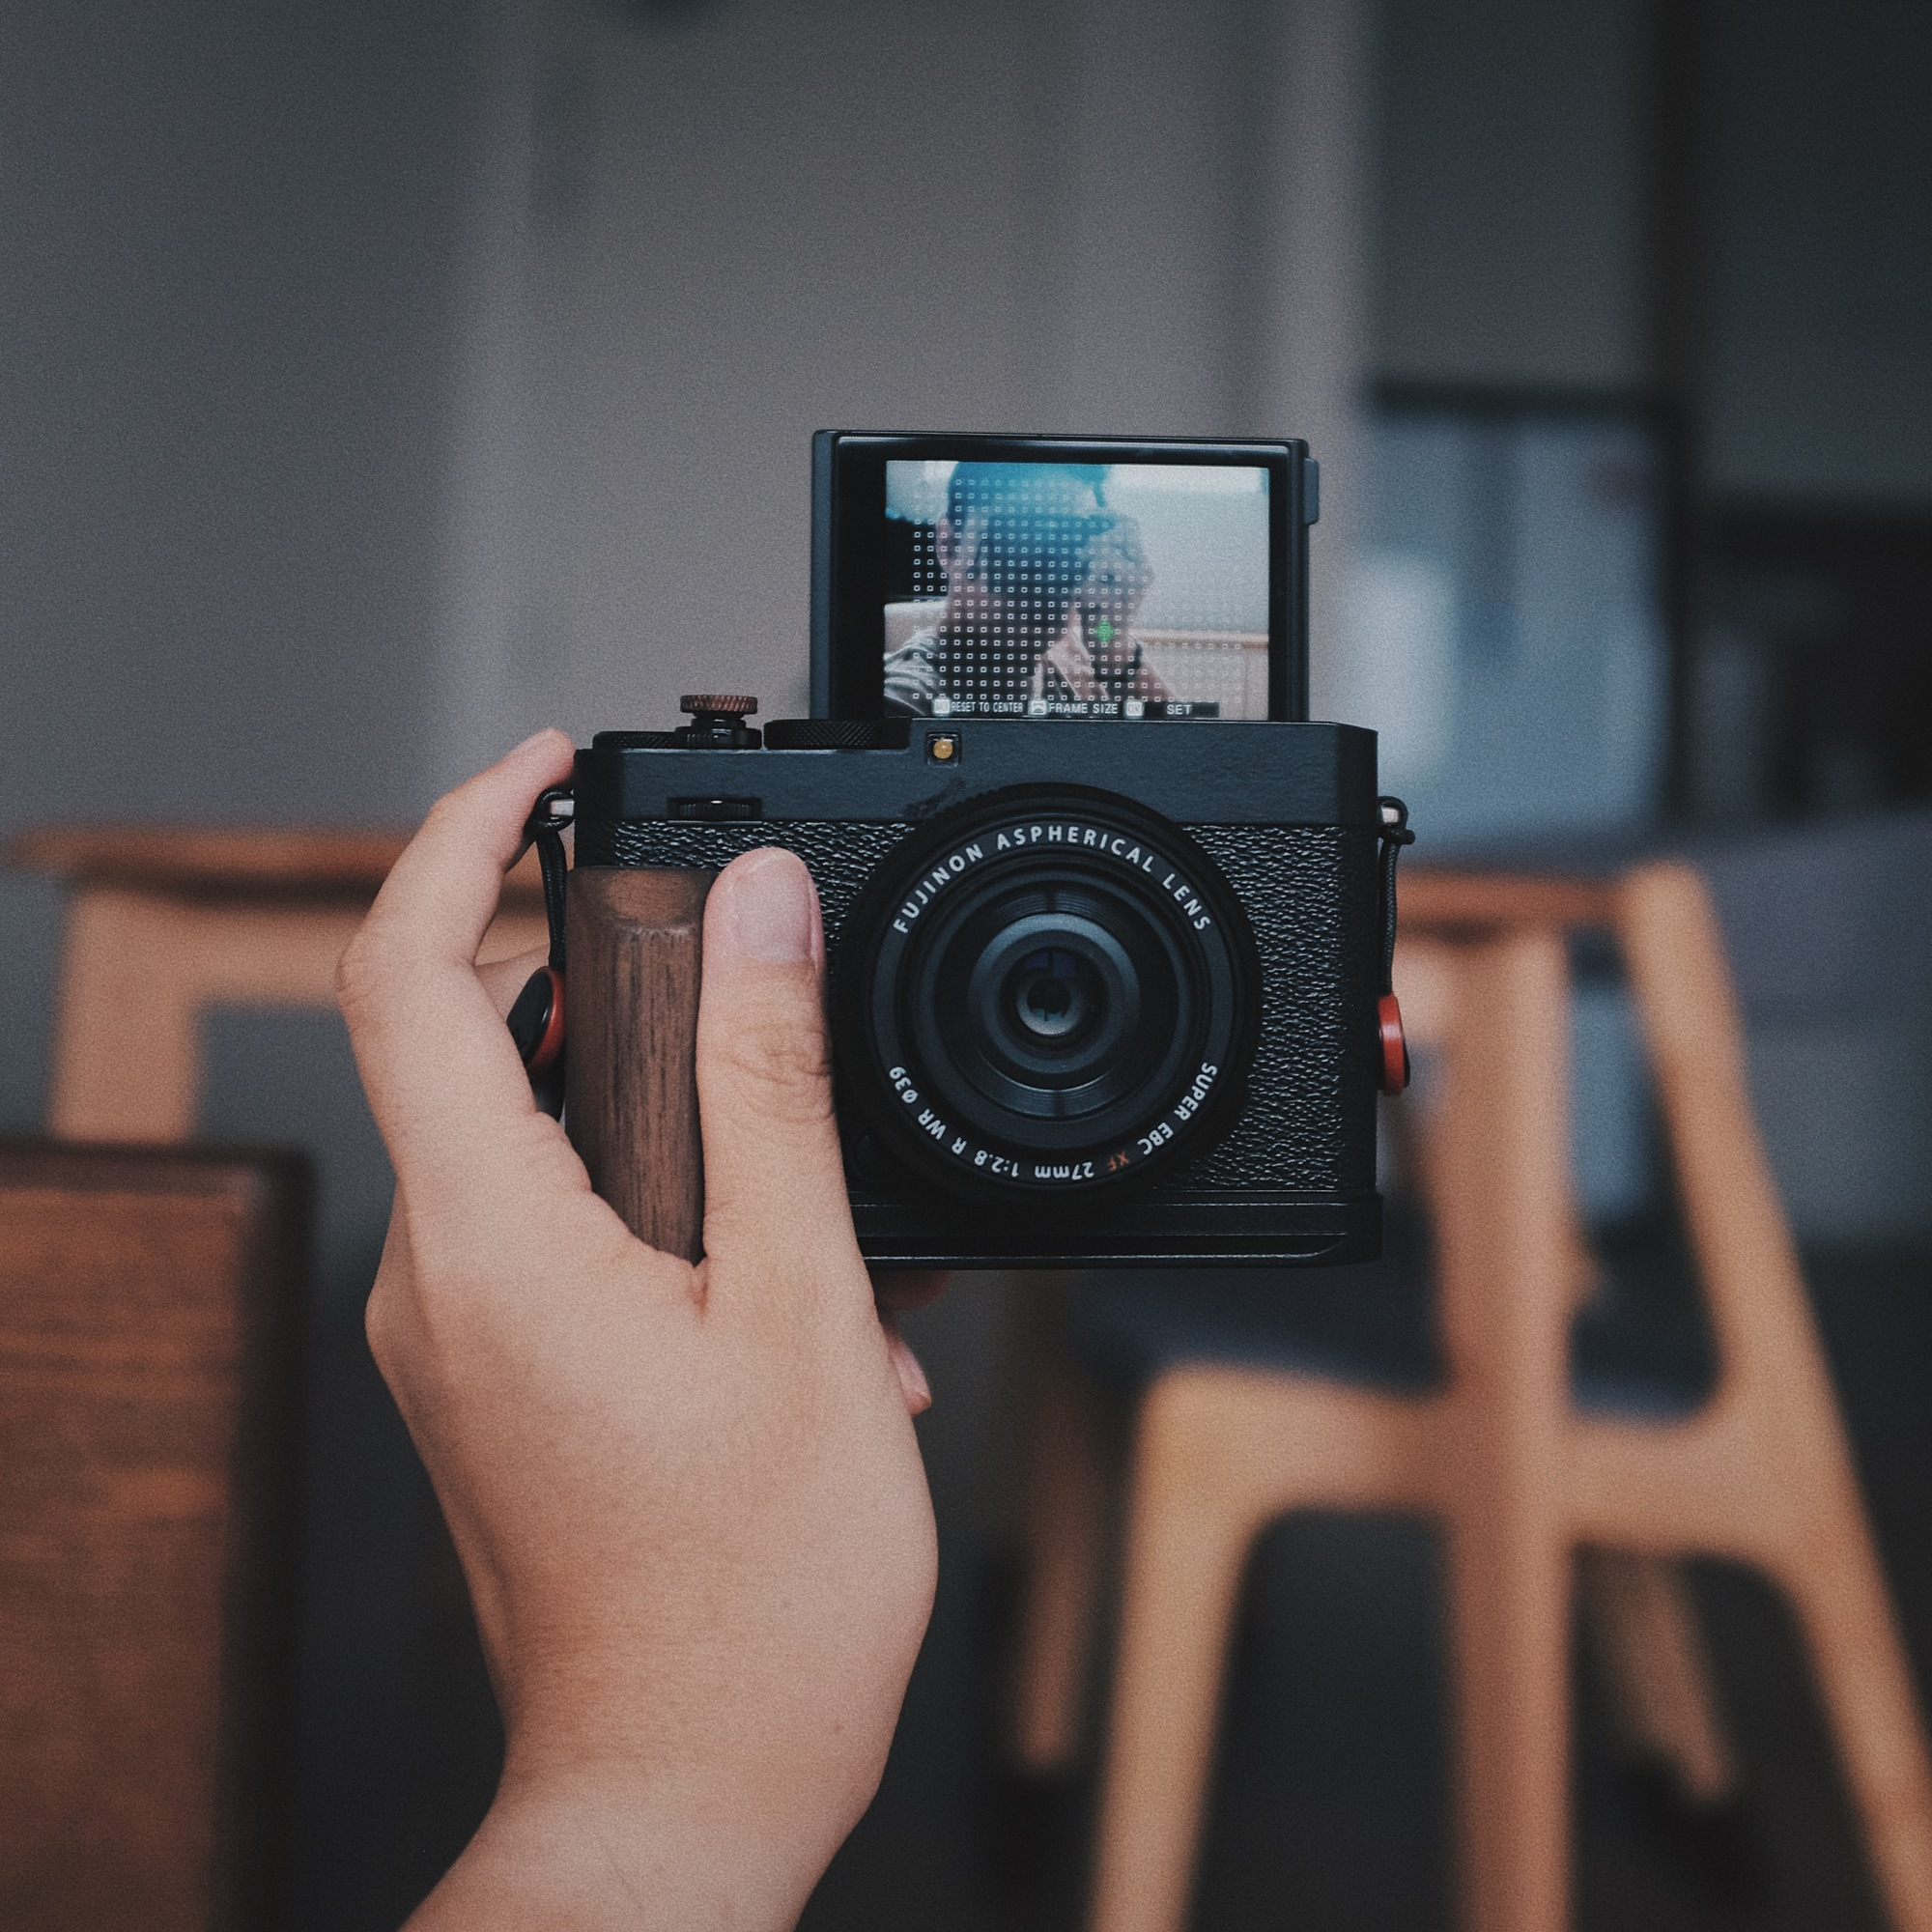
\includegraphics[width=\linewidth]{\envfinaldir/coverpic-prod.jpg}\par
            % \vskip 30pt
            \vfill

            \normalsize\rmfamily\scshape
            \copyright{} The Web Digest Project \hfill\large \envdatestr
        \end{center}
    \end{titlepage}
    % \restoregeometry
}
\newcommand{\simplehref}[1]{%
    \textcolor{blue!80!green}{\href{#1}{#1}}%
}
\renewcommand{\contentsname}{\center\Huge\sffamily\bfseries Contents\par\vskip 20pt}
\newcounter{ipartcounter}
\setcounter{ipartcounter}{0}
\newcommand{\ipart}[1]{
    % \vskip 20pt
    \clearpage
    \stepcounter{ipartcounter}
    \phantomsection
    \addcontentsline{toc}{chapter}{#1}
    % \begin{center}
    %     \Huge
    %     \sffamily\bfseries
    %     #1
    % \end{center}
    % \vskip 20pt plus 7pt
}
\newcounter{ichaptercounter}
\setcounter{ichaptercounter}{0}
\newcommand{\ichapter}[1]{
    % \vskip 20pt
    \clearpage
    \stepcounter{ichaptercounter}
    \phantomsection
    \addcontentsline{toc}{section}{\numberline{\arabic{ichaptercounter}}#1}
    \begin{center}
        \Huge
        \sffamily\bfseries
        #1
    \end{center}
    \vskip 20pt plus 7pt
}
\newcommand{\entrytitlefont}[1]{\subsection*{\raggedright\Large\sffamily\bfseries#1}}
\newcommand{\entryitemGeneric}[2]{
    % argv: title, url
    \parbox{\linewidth}{
        \entrytitlefont{#1}\par\vskip 5pt
        \footnotesize\ttfamily\mdseries
        \simplehref{#2}
    }\vskip 11pt plus 11pt minus 1pt
}
\newcommand{\entryitemGithub}[3]{
    % argv: title, url, desc
    \parbox{\linewidth}{
        \entrytitlefont{#1}\par\vskip 5pt
        \footnotesize\ttfamily\mdseries
        \simplehref{#2}\par\vskip 5pt
        \small\rmfamily\mdseries#3
    }\vskip 11pt plus 11pt minus 1pt
}
\newcommand{\entryitemAp}[3]{
    % argv: title, url, desc
    \parbox{\linewidth}{
        \entrytitlefont{#1}\par\vskip 5pt
        \footnotesize\ttfamily\mdseries
        \simplehref{#2}\par\vskip 5pt
        \small\rmfamily\mdseries#3
    }\vskip 11pt plus 11pt minus 1pt
}
\newcommand{\entryitemHackernews}[3]{
    % argv: title, hnurl, rawurl
    % \parbox{\linewidth}{
    %     \entrytitlefont{#1}\par\vskip 5pt
    %     \footnotesize\ttfamily\mdseries
    %     \simplehref{#3}\par
    %     \textcolor{black!50}{\href{#2}{#2}}
    % }\vskip 11pt plus 11pt minus 1pt
    \begin{minipage}{\linewidth}
            \entrytitlefont{#1}\par\vskip 5pt
            \footnotesize\ttfamily\mdseries
            \simplehref{#3}\par
            \textcolor{black!50}{\href{#2}{#2}}
    \end{minipage}\par\vskip 11pt plus 11pt minus 1pt
}







\begin{document}

\makeheader

\tableofcontents\clearpage




\ipart{Developers}
\ichapter{Hacker News}
\entryitemTwoLinks{"Anna, Lindsey Halligan Here." My Signal exchange with the interim U.S. attorney}{https://news.ycombinator.com/item?id=45662053}{https://www.lawfaremedia.org/article/anna--lindsey-halligan-here}

\entryitemTwoLinks{Replacing a \$3000/mo Heroku bill with a \$55/mo server}{https://news.ycombinator.com/item?id=45661253}{https://disco.cloud/blog/how-idealistorg-replaced-a-3000mo-heroku-bill-with-a-55-server/}

\entryitemTwoLinks{Doomsday scoreboard}{https://news.ycombinator.com/item?id=45661084}{https://doomsday.march1studios.com/}

\entryitemTwoLinks{Magit Is Amazing}{https://news.ycombinator.com/item?id=45659812}{https://heiwiper.com/posts/magit-is-awesome/}

\entryitemTwoLinks{ChatGPT Atlas}{https://news.ycombinator.com/item?id=45658479}{https://chatgpt.com/atlas}

\entryitemTwoLinks{Fallout from the AWS outage: Smart mattresses go rogue}{https://news.ycombinator.com/item?id=45658056}{https://quasa.io/media/the-strangest-fallout-from-the-aws-outage-smart-mattresses-go-rogue-and-ruin-sleep-worldwide}

\entryitemTwoLinks{The Programmer Identity Crisis}{https://news.ycombinator.com/item?id=45658019}{https://hojberg.xyz/the-programmer-identity-crisis/}

\entryitemTwoLinks{Build your own database}{https://news.ycombinator.com/item?id=45657827}{https://www.nan.fyi/database}

\entryitemTwoLinks{Public trust demands open-source voting systems}{https://news.ycombinator.com/item?id=45657431}{https://www.voting.works/news/public-trust-demands-open-source-voting-systems}

\entryitemTwoLinks{Is Sora the beginning of the end for OpenAI?}{https://news.ycombinator.com/item?id=45657428}{https://calnewport.com/is-sora-the-beginning-of-the-end-for-openai/}

\entryitemTwoLinks{Ask HN: Our AWS account got compromised after their outage}{https://news.ycombinator.com/item?id=45657345}{https://news.ycombinator.com/item?id=45657345}

\entryitemTwoLinks{Apple alerts exploit developer that his iPhone was targeted with gov spyware}{https://news.ycombinator.com/item?id=45657302}{https://techcrunch.com/2025/10/21/apple-alerts-exploit-developer-that-his-iphone-was-targeted-with-government-spyware/}

\entryitemTwoLinks{Foreign hackers breached a US nuclear weapons plant via SharePoint flaws}{https://news.ycombinator.com/item?id=45657287}{https://www.csoonline.com/article/4074962/foreign-hackers-breached-a-us-nuclear-weapons-plant-via-sharepoint-flaws.html}

\entryitemTwoLinks{AI is making us work more}{https://news.ycombinator.com/item?id=45656916}{https://tawandamunongo.dev/posts/2025/10/ai-work-more}

\entryitemTwoLinks{LLMs can get "brain rot"}{https://news.ycombinator.com/item?id=45656223}{https://llm-brain-rot.github.io/}

\entryitemTwoLinks{UA 1093}{https://news.ycombinator.com/item?id=45656044}{https://windbornesystems.com/blog/ua-1093}

\entryitemTwoLinks{Ilo – a Forth system running on UEFI}{https://news.ycombinator.com/item?id=45655263}{https://asciinema.org/a/Lbxa2w9R5IbaJqW3INqVrbX8E}

\entryitemTwoLinks{Our modular, high-performance Merkle Tree library for Rust}{https://news.ycombinator.com/item?id=45655190}{https://github.com/bilinearlabs/rs-merkle-tree}

\entryitemTwoLinks{NASA chief suggests SpaceX may be booted from moon mission}{https://news.ycombinator.com/item?id=45655188}{https://www.cnn.com/2025/10/20/science/nasa-spacex-moon-landing-contract-sean-duffy}

\entryitemTwoLinks{Neural audio codecs: how to get audio into LLMs}{https://news.ycombinator.com/item?id=45655161}{https://kyutai.org/next/codec-explainer}\ichapter{Phoronix}
\entryitemGeneric{\hskip 0pt{}AlmaLinux 10.1 Will Support The Btrfs File-System}{https://www.phoronix.com/news/AlmaLinux-10.1-Btrfs-Plans}

\entryitemGeneric{\hskip 0pt{}Valkey 9.0 Released With Ability To Achieve One Billion Requests / Second}{https://www.phoronix.com/news/Valkey-9.0-Released}

\entryitemGeneric{\hskip 0pt{}Intel Nova Lake To Feature 6th Gen NPU}{https://www.phoronix.com/news/Intel-Nova-Lake-6th-Gen-NPU}

\entryitemGeneric{\hskip 0pt{}Revisiting The SNC3 vs. HEX Mode Performance With Intel Xeon 6 Granite Rapids}{https://www.phoronix.com/review/intel-xeon-snc3-hex-benchmarks}

\entryitemGeneric{\hskip 0pt{}TARmageddon Strikes: High Profile Security Vulnerability In Popular Rust Library}{https://www.phoronix.com/news/Rust-TARmageddon}

\entryitemGeneric{\hskip 0pt{}More Kernel Graphics Driver \& Accelerator/NPU Driver Updates Ready For Linux 6.19}{https://www.phoronix.com/news/Linux-6.19-DRM-Misc-Next-2}

\entryitemGeneric{\hskip 0pt{}AMD PMF Linux Driver Working On AMD SystemDeck Support}{https://www.phoronix.com/news/AMD-PMF-Linux-SystemDeck}

\entryitemGeneric{\hskip 0pt{}Linux 6.19 Will Add Support For The Logitech G13 Keypad - 17 Years After Hardware Debut}{https://www.phoronix.com/news/Logitech-G13-For-Linux-6.19}

\entryitemGeneric{\hskip 0pt{}Blender 5.1 Aiming For Vulkan By Default, More Improvements Coming}{https://www.phoronix.com/news/Blender-5.1-Vulkan-Default}


\ipart{Developers~~~~(zh-Hans)}
\ichapter{Solidot}
\entryitemGeneric{\hskip 0pt{}SpaceX 进度滞后 NASA 可能选择其它公司开发月球着陆器}{https://www.solidot.org/story?sid=82600}

\entryitemGeneric{\hskip 0pt{}美国客机疑与气象气球发生碰撞}{https://www.solidot.org/story?sid=82599}

\entryitemGeneric{\hskip 0pt{}KDE Plasma 6.5 释出}{https://www.solidot.org/story?sid=82598}

\entryitemGeneric{\hskip 0pt{}中国东南沿海同时遭遇海平面加速上升和下沉}{https://www.solidot.org/story?sid=82597}

\entryitemGeneric{\hskip 0pt{}被切断大脑区域的脑电图与深度睡眠脑电图相似}{https://www.solidot.org/story?sid=82596}

\entryitemGeneric{\hskip 0pt{}SpaceX 发射了第 1 万颗 Starlink 卫星}{https://www.solidot.org/story?sid=82595}

\entryitemGeneric{\hskip 0pt{}Steam 平台一款游戏的愿望单数字越高是否销量越多?}{https://www.solidot.org/story?sid=82594}

\entryitemGeneric{\hskip 0pt{}零工正在训练会取代他们的技术}{https://www.solidot.org/story?sid=82593}

\entryitemGeneric{\hskip 0pt{}冰岛发现野外蚊子}{https://www.solidot.org/story?sid=82592}

\entryitemGeneric{\hskip 0pt{}FSF 呼吁 Windows 10 用户切换到 GNU/Linux}{https://www.solidot.org/story?sid=82591}

\entryitemGeneric{\hskip 0pt{}韦伯望远镜发现的小红点是什么?}{https://www.solidot.org/story?sid=82590}

\entryitemGeneric{\hskip 0pt{}Servo v0.0.1 释出}{https://www.solidot.org/story?sid=82589}

\entryitemGeneric{\hskip 0pt{}AWS 宕机影响亚马逊和《堡垒之夜》等游戏}{https://www.solidot.org/story?sid=82588}

\entryitemGeneric{\hskip 0pt{}Xubuntu 官网被嵌入窃取加密货币的恶意程序}{https://www.solidot.org/story?sid=82587}

\entryitemGeneric{\hskip 0pt{}Windows 11 更新破坏了 Recovery Environment}{https://www.solidot.org/story?sid=82586}

\entryitemGeneric{\hskip 0pt{}日本电商巨头 ASKUL 遭勒索软件攻击}{https://www.solidot.org/story?sid=82585}

\entryitemGeneric{\hskip 0pt{}GIMP 正式提供 Snap 打包的版本}{https://www.solidot.org/story?sid=82584}

\entryitemGeneric{\hskip 0pt{}英伟达展示首块美制 Blackwell 芯片}{https://www.solidot.org/story?sid=82583}

\entryitemGeneric{\hskip 0pt{}7-Zip 远程代码执行漏洞 PoC 公开}{https://www.solidot.org/story?sid=82582}

\entryitemGeneric{\hskip 0pt{}GPT-5 并不能证明未解决的数学问题 }{https://www.solidot.org/story?sid=82581}\ichapter{V2EX}
\entryitemGeneric{\hskip 0pt{}[Java] 用 AI 生成了一个框架代码文档,真的很专业}{https://www.v2ex.com/t/1167448}

\entryitemGeneric{\hskip 0pt{}[iPhone] iPhone 播放微博视频弹幕卡顿}{https://www.v2ex.com/t/1167447}

\entryitemGeneric{\hskip 0pt{}[分享发现] OpenAI 发布 ChatGPT Atlas,浏览器正式进入 AI 时代了。}{https://www.v2ex.com/t/1167443}

\entryitemGeneric{\hskip 0pt{}[问与答] 有没有 Ontology 的大神}{https://www.v2ex.com/t/1167442}

\entryitemGeneric{\hskip 0pt{}[分享发现] 一款基于维基百科的侦探游戏}{https://www.v2ex.com/t/1167441}

\entryitemGeneric{\hskip 0pt{}[Apple] 分享一款 iOS 影视变身软件}{https://www.v2ex.com/t/1167440}

\entryitemGeneric{\hskip 0pt{}[宽带症候群] 成都联通给了个华为星光 F50 尊享版,这玩意如何}{https://www.v2ex.com/t/1167438}

\entryitemGeneric{\hskip 0pt{}[分享发现] 双 11 购物咨询,喷友们对于筋膜枪的推荐}{https://www.v2ex.com/t/1167436}

\entryitemGeneric{\hskip 0pt{}[路由器] iKuai 的企业级路由相较于 tplink 等有什么优势}{https://www.v2ex.com/t/1167435}

\entryitemGeneric{\hskip 0pt{}[Go 编程语言] golang.org/x/sync/syncmap 被 struct 裹挟时 使用前为什么必须为每个键初始化 不然取值得到 nil}{https://www.v2ex.com/t/1167432}

\entryitemGeneric{\hskip 0pt{}[问与答] 朋友们,技术网站的技术问题,刷不到新帖子的话,欢迎来交流下}{https://www.v2ex.com/t/1167431}

\entryitemGeneric{\hskip 0pt{}[推广] Hstock 数字商品电商平台提供成品账户,订阅与不同服务。分享可靠网站}{https://www.v2ex.com/t/1167430}

\entryitemGeneric{\hskip 0pt{}[分享创造] 图片转素描 AI 小工具}{https://www.v2ex.com/t/1167429}

\entryitemGeneric{\hskip 0pt{}[问与答] glm4.6 太难用了,跟 cc 比起来}{https://www.v2ex.com/t/1167428}

\entryitemGeneric{\hskip 0pt{}[London] 这个节点十年没更新了,来冒个泡,交个朋友}{https://www.v2ex.com/t/1167427}

\entryitemGeneric{\hskip 0pt{}[酷工作] 代招,成都桌面软件开发}{https://www.v2ex.com/t/1167426}

\entryitemGeneric{\hskip 0pt{}[问与答] 做了一个概率类的小游戏,被人攻击了,大家有没有什么好的防范手段}{https://www.v2ex.com/t/1167425}

\entryitemGeneric{\hskip 0pt{}[求职] [求职] 远程工作}{https://www.v2ex.com/t/1167424}

\entryitemGeneric{\hskip 0pt{}[Mac mini] lm studio 上部署哪个 ai 模型可以处理 pdf 文件啊?}{https://www.v2ex.com/t/1167422}

\entryitemGeneric{\hskip 0pt{}[问与答] 速冻食品里面为什么有那么多科技与狠活?}{https://www.v2ex.com/t/1167421}

\entryitemGeneric{\hskip 0pt{}[深圳] 又到了双十一和深圳换季的时候,求服装店推荐}{https://www.v2ex.com/t/1167420}

\entryitemGeneric{\hskip 0pt{}[互联网] 为什么提供 webdav 的网盘这么少?}{https://www.v2ex.com/t/1167419}

\entryitemGeneric{\hskip 0pt{}[硬件] 论坛里有用过锐捷家的 RG-EG310XS-E 的吗?}{https://www.v2ex.com/t/1167418}

\entryitemGeneric{\hskip 0pt{}[宽带症候群] 求教电信 hn8145xr 通过不了 itms 手动配置也无法获取 ip 了}{https://www.v2ex.com/t/1167417}

\entryitemGeneric{\hskip 0pt{}[程序员] 有人在工作中用 jsonnet 吗}{https://www.v2ex.com/t/1167416}

\entryitemGeneric{\hskip 0pt{}[问与答] 我的恋爱观念是否有问题?}{https://www.v2ex.com/t/1167415}

\entryitemGeneric{\hskip 0pt{}[Cloudflare] cloudflare 域名解析错误问题}{https://www.v2ex.com/t/1167414}

\entryitemGeneric{\hskip 0pt{}[分享创造] [技术分享] 我把斯坦福最新的 ACE 框架思想,做成了一个能让 Claude"自主进化"的开源 Playbook,结果有点超现实…}{https://www.v2ex.com/t/1167413}

\entryitemGeneric{\hskip 0pt{}[全球工单系统] clarity 的 real time 失效了吗}{https://www.v2ex.com/t/1167412}

\entryitemGeneric{\hskip 0pt{}[生活] 不买车,通勤和出行只打车的话, 有太多的局限}{https://www.v2ex.com/t/1167410}

\entryitemGeneric{\hskip 0pt{}[YouTube] 土区 IOS 家庭组订阅被取消,无法续订}{https://www.v2ex.com/t/1167409}

\entryitemGeneric{\hskip 0pt{}[问与答] PDD 砍单问题}{https://www.v2ex.com/t/1167408}

\entryitemGeneric{\hskip 0pt{}[Docker] Docker Compose 创建容器实例报错}{https://www.v2ex.com/t/1167406}

\entryitemGeneric{\hskip 0pt{}[Bitcoin] 这波行情结束了吗,要等 4 年了?}{https://www.v2ex.com/t/1167405}

\entryitemGeneric{\hskip 0pt{}[程序员] 为什么代码会腐败?原本好好的代码是怎么烂透的?}{https://www.v2ex.com/t/1167404}

\entryitemGeneric{\hskip 0pt{}[酷工作] Java 后端 \& 前端开发工程师(技术栈前沿, AI 落地实践,团队年轻有活力!)}{https://www.v2ex.com/t/1167403}

\entryitemGeneric{\hskip 0pt{}[程序员] Stocks AI 积分福利}{https://www.v2ex.com/t/1167402}

\entryitemGeneric{\hskip 0pt{}[iOS] iOS 26 是我用过的 iOS 大版本中影响日常使用 BUG 最多的一个版本。}{https://www.v2ex.com/t/1167401}

\entryitemGeneric{\hskip 0pt{}[Faucet] 赛博乞讨,感谢大佬}{https://www.v2ex.com/t/1167400}

\entryitemGeneric{\hskip 0pt{}[Solana] 今晚看好索拉拉什么行情?}{https://www.v2ex.com/t/1167399}

\entryitemGeneric{\hskip 0pt{}[分享创造] 做了个小程序,查找附近的乒乓球场地和球友。球友们来试试?}{https://www.v2ex.com/t/1167398}

\entryitemGeneric{\hskip 0pt{}[分享发现] 买了 iphone17 pro,最终还是叛变了!}{https://www.v2ex.com/t/1167397}

\entryitemGeneric{\hskip 0pt{}[问与答] 有没有人跟我一样一到医院量血压就高血压的}{https://www.v2ex.com/t/1167396}

\entryitemGeneric{\hskip 0pt{}[问与答] [买车]30 岁生日,我给父母买了辆车作为礼物}{https://www.v2ex.com/t/1167395}

\entryitemGeneric{\hskip 0pt{}[软件] 滴答清单被 Gooogle play 识别成有害应用}{https://www.v2ex.com/t/1167394}

\entryitemGeneric{\hskip 0pt{}[问与答] 双十一买什么会员,怎么划算?}{https://www.v2ex.com/t/1167393}

\entryitemGeneric{\hskip 0pt{}[分享创造] 个人用户对 IM 软件有用户需求吗}{https://www.v2ex.com/t/1167392}

\entryitemGeneric{\hskip 0pt{}[分享发现] 来 v2 差不多 3 年了 终于有 1 金币了!}{https://www.v2ex.com/t/1167390}

\entryitemGeneric{\hskip 0pt{}[macOS] mac os 26.1 beta 千万不要手欠升级啊}{https://www.v2ex.com/t/1167389}

\entryitemGeneric{\hskip 0pt{}[全球工单系统] 申请 Stripe 的微信支付时,它们似乎把内部流程邮件发出来了}{https://www.v2ex.com/t/1167388}


\ipart{Generic News}







\clearpage
\leavevmode\vfill
\footnotesize

Copyright \copyright{} 2023-2025 Neruthes and other contributors.

This document is published with CC BY-NC-ND 4.0 license.

The entries listed in this newsletter may be copyrighted by their respective creators.

This newsletter is generated by the Web Digest project.

The newsletters are also delivered via Telegram channel \CJKunderline{\href{https://t.me/webdigestchannel}{https://t.me/webdigestchannel}}.\\
RSS feed is available at \CJKunderline{\href{https://webdigest.pages.dev/rss.xml}{https://webdigest.pages.dev/rss.xml}}.

This newsletter is available in PDF at
\CJKunderline{\href{https://webdigest.pages.dev/}{https://webdigest.pages.dev/}}.

The source code being used to generate this newsletter is available at\\
\CJKunderline{\href{https://github.com/neruthes/webdigest}{https://github.com/neruthes/webdigest}}.

This newsletter is also available in
\CJKunderline{\href{http://webdigest.pages.dev/readhtml/\envyear/WebDigest-20251022.html}{HTML}} and
\CJKunderline{\href{https://github.com/neruthes/webdigest/blob/master/markdown/\envyear/WebDigest-20251022.md}{Markdown}}.


\coverpic{https://unsplash.com/photos/sunbeams-break-through-clouds-over-distant-mountains-oRoRQZuB6tk}{Zach Kessinger}


\end{document}
